\section{Spring-Mass System}
\label{sec:Appendix1}
\subsection{Introduction}
The cerebral cortex consists of a convoluted surface of gyri and sulci. There are accurate models for the gyrification of the cortex as a whole \cite{Tallinen2014} and there is a description of how the layers within the cortex behave \cite{Bok1929}: the volume ratio between layers is equal for an arbitrarily curved pieced of cerebral cortex. This is what has become known as the Bok-principle. Here we describe how to simulate data for a two dimensional system that obeys Bok's principle by means of a spring-mass system. A spring-mass system was chosen, because it is independent of the algorithms by means of which we estimate curvature in the volume. This makes it ideal benchmark data for the methods presented in the body of this paper.

\subsection{Spring-Mass System}
The cortex is modelled by means of a spring mass system. This is an approximation of the cortex consisting of quadrilaterals. Each quadrilateral consists of four edges and four vertices, which are the springs and masses respectively. The collection of springs and masses that form quadrilaterals will henceforth be referred to as the system.

The system has total energy $U$. In the present simulation only a single contribution to the energy is considered, related to the area of each quadrilateral. More generally, other contributions could be taken into account, for example relating to the length of each edge:
\begin{equation}
U=U_{area}+U_{edge}+...
\end{equation}
We are looking for the case where the energy is minimised, as this is when the system has come to rest and all quadrilaterals have reached an equilibrium area. Note that only the vertices are displaced in the first instance; the edges and quadrilaterals are formed as a consequence. The energy decreases by moving the vertices in the direction of the net force applied to them. The force $\vec{F}_n$ on vertex $n$ is minus the derivative of $U$ with respect to the position $\vec{r}_n$ of that vertex: 
\begin{equation}
\vec{F}_n= -\nabla_n U.
\label{Forces}
\end{equation}

% \subsubsection{Area force}
A quadrilateral $Q_i$ is defined to be the space enclosed by four vertices in two dimensions  $\vec{u_i}$, $\vec{v_i}$, $\vec{w_i}$ and $\vec{k_i}$, shown in Figure~\ref{Tetrahedron}.
\begin{figure}[ht]
\begin{center}
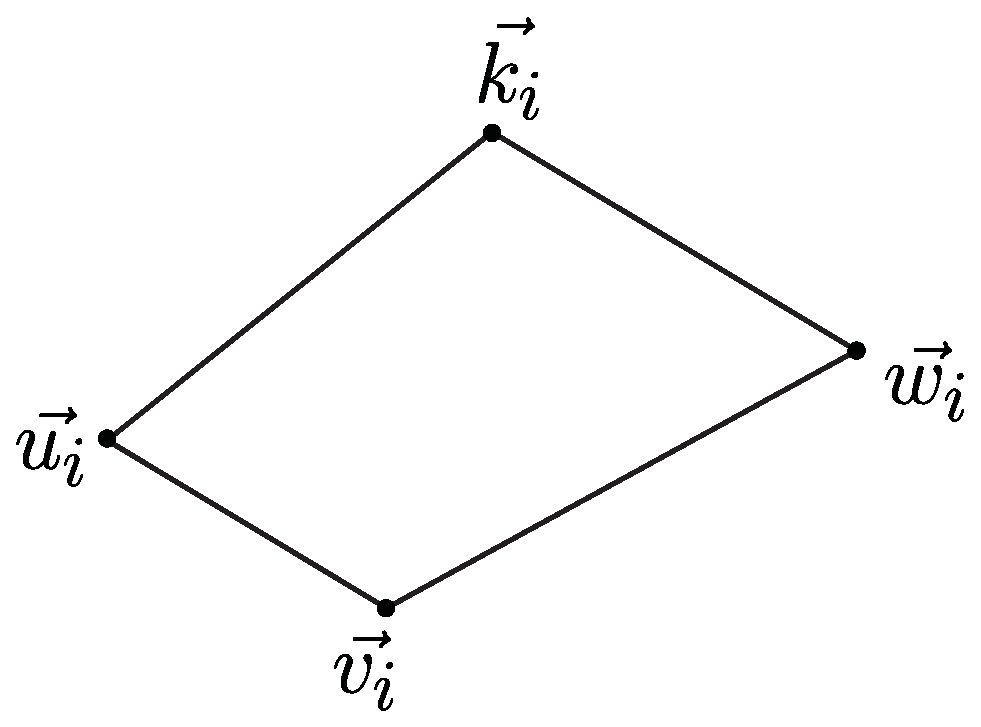
\includegraphics[width=0.33\textwidth, clip=true]{./Chapters/03_GLM/./Images/Quadrilateral} 
\caption{Quadrilateral $Q_i$, consisting of vertices $\vec{u_i}$, $\vec{v_i}$, $\vec{w_i}$ and $\vec{k_i}$.}
\label{Tetrahedron}
\end{center}
\end{figure}
Its area $A_i$ is a scalar function depending on the vertices of the quadrilateral,~$A_i=A_i(\vec{u}_i, \vec{v}_i, \vec{w}_i, \vec{k}_i)$: 
\begin{eqnarray}
A_i&=&\frac{1}{2}
[\left( u_{i,y} v_{i,x} - u_{i,x} v_{i,y} \right) + \left( v_{i,y} w_{i,x} - v_{i,x} w_{i,y} \right) + \textellipsis \\
& & \left( w_{i,y} k_{i,x} - w_{i,x} k_{i,y} \right) + \left( k_{i,y} u_{i,x} - k_{i,x} u_{i,y} \right) ]
\label{areaQ}
\end{eqnarray}
The vertices $\vec{u_i}$, $\vec{v_i}$, $\vec{w_i}$ and $\vec{k_i}$ are chosen such that $A_i > 0$.

Let $Q = \{Q_1, Q_2, Q_3, ...\}$ be the set of all quadrilaterals. The energy of the system is
\begin{equation}
U=U_{area}=\sum\limits_{Q_i\in Q}U_i
\end{equation}
where $U_i$ is the energy of quadrilateral $Q_i$
\begin{equation}
U_i=\frac{1}{2}k_A \left(A_i-A_0\right)^2
\end{equation}
such that the quadrilateral energy is a function of the difference between the actual area $A_i$ and the equilibrium area $A_0$. 

Subsequently, the gradient is computed for the energy stored in the system:
\begin{equation}
\nabla_n U_{area}=\nabla_n \sum\limits_{Q_i\in \vec{Q}} U_i=\sum\limits_{Q_i\in Q} \nabla_n U_i.
\end{equation}
The gradient of a single quadrilateral energy term takes the form:
\begin{equation}
\nabla_n U_{i} = \nabla_n \frac{1}{2}k_A\left(A_i-A_0\right)^2 = k_A \left(A_i-A_0\right) \nabla_n A_i.
\label{EnergyLaplacian}
\end{equation}
Note that $\nabla_n U_{i}$ can be non-zero only if vertex $n$ belongs to $Q_n$, i.e. if $\vec{r}_n$ is one of the vertices $\vec{u_i}$, $\vec{v_i}$, $\vec{w_i}$ or $\vec{k_i}$. To be explicit, let $\vec{r}_n = \vec{u_i}$. In two dimensions $\nabla_n A_i = ( \frac{\partial A_i}{\partial u_{i,x}}, \frac{\partial A_i}{\partial u_{i,y}} )$. The two components follow immediately from \ref{areaQ}:
\begin{eqnarray}
\frac{\partial A_i}{\partial u_{i,x}}&=&
\frac{1}{2} \left( k_{i,y} - v_{i,y} \right),
\nonumber \\
\frac{\partial A_i}{\partial u_{i,y}}
&=&
\frac{1}{2} \left( v_{i,x} - k_{i,x} \right).
\label{uglypartialderivatives}
\end{eqnarray}

Combining equations~\ref{Forces}, \ref{EnergyLaplacian} and \ref{uglypartialderivatives}, the resulting force on vertex $n$ due to the preservation of volume is
\begin{equation}
\vec{F}_n = \sum\limits_{Q_i \ni n} -\frac{1}{2}k_A (A_0-A_i) \left( k_{i,y} - v_{i,y}, v_{i,x} - k_{i,x}\right).
\end{equation}
Here the summation is over the quadrilaterals $Q_i$ that contain vertex $n$, and $\vec{k}_i$ and $\vec{v}_i$ are the neighbours of $\vec{r}_n$ in $Q_i$. The vertex will come to rest if $A_i=A_0$, and the strength of the force can be adjusted by parameter $k_A$. All forces are additive.


This was implemented in C\texttt{++} as a stand-alone application. The program reads in a mesh and evolves the vertices until the system comes to rest. 
